\section{Lecture 1. Introduction to Mathematical Method in VDA}


Introduction

the fourth industrial revolution
computer vision 

\subsection{Intelligent Vision System}
    \subsubsection{The concept of Intelligence}
        Some indications of intelligence that are of interest include:
        \begin{itemize}
            \item memory, recall, creativity
            \item computation, inference, recognition, prediction
            \item retrieval, localization \& moving, reasoning
        \end{itemize}
    \subsubsection{The intelligence levels of Vision System's output}
    \subsubsection{The three basic levels of Vision Systems:}
    \begin{itemize}
        \item Basic methods for data processing\\
        \textbf{Q: Những khám phá nào ở cấp độ 1 mà làm thay đổi ngoạn mục cấp độ 2 và 3?}\\
        A: Fast Fourier Transform (FFT) and Convolutional Neural Network (CNN).
        \item Single task processing
        \item Complex applications processing. 
    \end{itemize}
    \subsubsection{Some Intelligent Vision Systems}
    \begin{itemize}
        \item Intelligent Transportation System (ITS)
        \item Intelligent Monitor System (IMS)
        \item Autonomous Vehicle System (AVS)
        \item Fault Inspection System (FIS)
        \item Disease Diagnosis System based on Imaging
        \item Harvesting System in Agriculture
        \item Intelligent Image-Video Retrieval
    \end{itemize}
    \subsubsection{Learning Method}
    Everything advances slowly 
    Ngta sẽ nghiên cứu các mô hình học máy để cải tiến hơn nữa.
    \begin{itemize}
        \item Supervised learning (semi-, self-)
        \item Unsupervised learning
        \item Reinforcement learning: học tăng cường, nổi lên thông qua AlphaGo, bây giờ ứng dụng trong xe tự hành, ChatGPT,...
        RL is a machine learning technique that focouses on training and algorithm following the cut-and-try approach. The algotirithm 
        \begin{itemize}
            \item The agent or the learner
            \item The environment
        \end{itemize}
        Examples:
        \begin{itemize}
            \item any real-world problem where an agent must interact with an uncertain environment to meet a specific goal: robotics, AlphaGo, autonomous driving, logistics,...
        \end{itemize}
        Benefits:
        \begin{itemize}
            \item Artificial General Intelligence (AGI)
            \item does not need a separate data collection step
        \end{itemize}
        \item Continual learning: học
        \item Federated learning
        \item Deep learning
        \item Transfer learning
        \item Meta learning
        Deep neural networks can achieve great succes when presented wiht large datasets and sufficient computational resources. However, their ability to learn new concepts quickly is limited. It is one of the defining aspects of human intelligence (Jankowski, 2018).\\
        Meta learning is one approach to this issue by enabling the network to learn how to learn.\\
        \begin{itemize}
            \item Image Classification
            \item Facial Recognition and Face Antispoofing
            \item Person-specific talking head generateion for unseen 
        \end{itemize}
    \end{itemize}

    Traditional Programming
    data
            -> computer -> results
    set of rules (proram)
        
    Machine Learning
    data
            -> computer -> set of rules (model)
    results (Optional)
\\
    Machine learning as a field is "concerned with the question of how to construct computer programs that automatically improve with experience." - Tom Mitchell
    1997 he presents the formal definition of machine learning as follows:\\
    "A computer program is said to learn from \textbf{experience E} with respect to some \textbf{class of tasks T} and \textbf{performance measure P}, if its performance at tasks in T, as measured by P, improves with experience E."\\
    There are three main machine learning paradigms:
    \begin{itemize}
        \item Supervised learning: learning properties of data using labelled data
        \item Unsupervised learning: learning properties of data using unlabelled data
        \item Reinforcement learning: learning properties of an environment through trial and error 
    \end{itemize}




learning Method


advanced deep neural network system
advanced deep neural network architecture
\begin{itemize}
    \item Le-Net, AlexNet, VGG, GoogleNet
    \item ResNet, SeNet, EfficientNet
    \item Graph Neural Network (GNN)
    \item Generative Adversarial Network (GAN)
    \item Vision Transformer (ViT)
\end{itemize}

\textbf{Q: Có mạng học máy nào mới gần đây không?}\\
A: 
\begin{itemize}
    \item \textbf{Swin Transformer}: Một loại mạng Transformer được thiết kế cho các tác vụ thị giác máy tính, nổi bật với khả năng xử lý hình ảnh hiệu quả và chính xác.
    \item \textbf{MLP-Mixer}: Một kiến trúc mạng mới sử dụng các lớp MLP (Multi-Layer Perceptron) để trộn các đặc trưng không gian và kênh, thay vì sử dụng các lớp convolution.
    \item \textbf{ConvNeXt}: Một biến thể hiện đại của mạng convolutional neural network (CNN) truyền thống, được thiết kế để cạnh tranh với các mô hình Transformer trong các tác vụ thị giác.
    \item \textbf{DALL-E 2}: Một mô hình học sâu của OpenAI có khả năng tạo ra hình ảnh từ mô tả văn bản, cải tiến từ phiên bản DALL-E ban đầu.
    \item \textbf{CLIP}: Một mô hình của OpenAI kết hợp giữa hình ảnh và văn bản, cho phép hiểu và tạo ra các mô tả văn bản từ hình ảnh và ngược lại.
\end{itemize}


\subsection{Generative AI}
\subsubsection{Generative AI in Computer Vision}
\begin{itemize}
    \item Generative model
    \begin{itemize}
        \item GAN
        \item DIFFUSION
    \end{itemize}
    \item Image-tasks
    \begin{itemize}
        \item Text2Image, Image2Text
        \item Style2Image
        \item HumanBrainSignal2Image
    \end{itemize}
    \item Video-tasks
    \begin{itemize}
        \item Text2Video, Video2Text
        \item Text2Animation
    \end{itemize}
    \item Computer Graphics-tanks
    \begin{itemize}
        \item Text23DScene
        \item Text23DObjectAnimation
    \end{itemize}
\end{itemize}
\textbf{Q: Ví dụ về lĩnh vực, chủ đề mà Generative AI có thể hỗ trợ, không có không được}

A: Image2Text (e.g. tóm tắt video)



\subsubsection{Diffusion Model}


"Diffusion Models are a class of probabilistic generative models that turn noise to a representative data sample."

Using Diffusion models, we can generate images either conditionally or unconditionally.

1. Unconditional image generation simply means that the model converts noise into any "random representative data sample." The generation process is not controlled or guided, and the model can generate an image of any nature.


\textbf{Q: Nếu như đánh context "flamingos standing on water, red sunset, pink-red water reflection" thì máy có generate được hình ảnh khác không?}\\
A: Có, các mô hình học sâu hiện đại như DALL-E 2 của OpenAI có khả năng tạo ra hình ảnh từ mô tả văn bản. Khi cung cấp mô tả như "flamingos standing on water, red sunset, pink-red water reflection", mô hình có thể tạo ra một hình ảnh tương ứng với mô tả này. Các mô hình này sử dụng các kỹ thuật tiên tiến trong học sâu và xử lý ngôn ngữ tự nhiên để hiểu và chuyển đổi mô tả văn bản thành hình ảnh.

\begin{itemize}
    \item \textbf{DALL-E 2}: Một mô hình học sâu của OpenAI có khả năng tạo ra hình ảnh từ mô tả văn bản. Với mô tả "flamingos standing on water, red sunset, pink-red water reflection", DALL-E 2 có thể tạo ra một hình ảnh với các đặc điểm như vậy.
    \item \textbf{Imagen}: Một mô hình của Google cũng có khả năng tương tự, tạo ra hình ảnh từ mô tả văn bản với độ chính xác và chi tiết cao.
\end{itemize}

Các mô hình này đã được huấn luyện trên hàng triệu cặp hình ảnh và mô tả văn bản, giúp chúng có khả năng hiểu và tạo ra hình ảnh từ các mô tả phức tạp.


\textbf{Q: mỗi lần tôi gõ cùng một câu thì nó ra một kết quả khác nhau hay giống nhau?}\\
A: tuỳ vào model


\textbf{Q: Nếu Intelligence System chỉ dừng ở mức thông minh mà không phải ở mức thông tuệ thì sẽ dừng ở lĩnh vực nào?}\\
A: Nó sẽ chủ yếu dừng lại ở các lĩnh vực yêu cầu khả năng xử lý thông tin và ra quyết định dựa trên các quy tắc và dữ liệu có sẵn, nhưng không yêu cầu sự hiểu biết sâu sắc, khả năng suy luận phức tạp, hoặc khả năng đưa ra các quyết định mang tính chiến lược và đạo đức. Cụ thể bao gồm:
\begin{itemize}
    \item \textbf{Tự động hóa và điều khiển}: Các hệ thống thông minh có thể thực hiện các nhiệm vụ tự động hóa trong sản xuất, quản lý năng lượng, và điều khiển các thiết bị điện tử.
    \item \textbf{Xử lý ngôn ngữ tự nhiên}: Các ứng dụng như dịch máy, nhận dạng giọng nói, và chatbot có thể hoạt động hiệu quả mà không cần đến mức độ thông tuệ cao.
    \item \textbf{Phân tích dữ liệu}: Các hệ thống thông minh có thể phân tích dữ liệu lớn để tìm ra các mẫu và xu hướng, hỗ trợ ra quyết định trong kinh doanh và tiếp thị.
    \item \textbf{Thị giác máy tính}: Nhận dạng hình ảnh và video, phát hiện đối tượng, và phân loại hình ảnh là những nhiệm vụ mà hệ thống thông minh có thể thực hiện tốt.
    \item \textbf{Hệ thống khuyến nghị}: Các hệ thống này có thể đề xuất sản phẩm, dịch vụ, hoặc nội dung dựa trên sở thích và hành vi của người dùng.
\end{itemize}

Tuy nhiên, để đạt được mức thông tuệ, hệ thống cần có khả năng hiểu biết sâu sắc, suy luận phức tạp, và đưa ra các quyết định mang tính chiến lược và đạo đức, điều này đòi hỏi sự phát triển vượt bậc trong các lĩnh vực như trí tuệ nhân tạo tổng quát (AGI) và học sâu (deep learning).

An idea used in non-equilibrium statistical physics is that we can \textbf{gradually convert one distribution into another}. In 2015, Sohl-Dicktein et al., inspired by this, created "Diffusion Probabilistic models" or "Diffusion models" in short, building on this essential idea.

They build - \textbf{"A generative Markov chain which converts a simple known distribution (e.g., a Gaussian) into a target (data) distribution using a diffusion process."}

\begin{figure}[H]
    \centering
    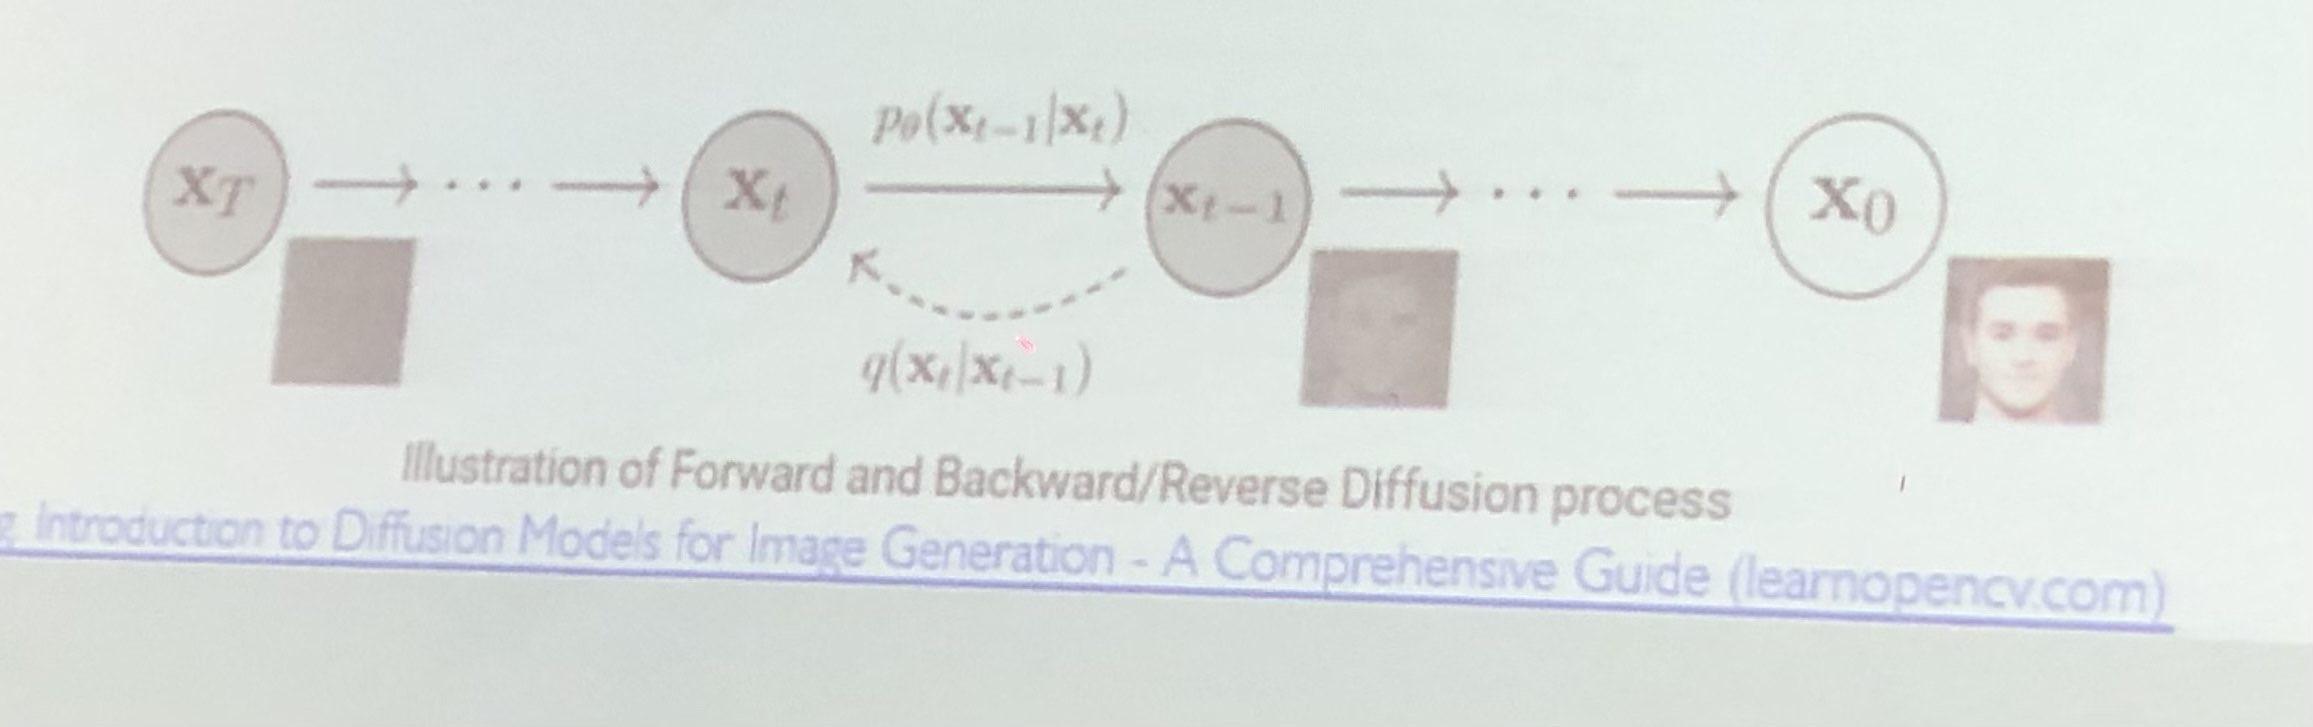
\includegraphics[scale=.2]{img/ForwardNBackwardORReverse Diffusion process.jpg}
    \caption{Illustration of Forward and Backward/Reverse Diffusion process}
    \label{fig:my_label_with_H}
\end{figure}

\textbf{In 2015}, Sohl-Dickstein et al. published paper "Deep Unsupervised Learning using Nonequilibrium Thermodynamics" and Diffusion models in deep learning were first introduced.

\textbf{In 2019}, Song et al. published a paper, "Generative Modeling by Estimating Gradients of the Data Distribution," using the same principle but a different approach.

\textbf{In 2020}, Ho et al. published the paper, now-popular "Denoising Diffusion Probabilistic Models" (DDPM for short).

\textbf{After 2020}, research in diffusion models took off. Much progress has been made in creating, training, and improving diffusion-based generative modeling in a relatively short time.

Some of the Diffusion-based Image Generation models that became famous over the past few months.

Some typical famous Diffusion-based Image Generation models include:
\begin{itemize}
    \item \textbf{DALL-E 2} by OpenAI
    \item \textbf{Imagen} by Google
    \item \textbf{Stable Diffusion} by StabilityAI
    \item \textbf{Midjourney}
\end{itemize}

D and G play the following two-player minimax game with value function $V (G, D)$:

\begin{equation*}
    \min_{G} \max_{D} V(D,G) = \mathbb{E}_{x \sim p_{\text{data}}(x)}[\log D(x)] + \mathbb{E}_{z \sim p_{z}(z)}[\log(1 - D(G(z)))]
\end{equation*}

Discriminator output for real data x

Discriminator output for generated fake data G(z)

Min Max V(D,G) = Ex-Plate [logD(x)] + Ez-P2(2) [log(1 – D(G(z)))] G

Error from the discriminator model training

Error from the combined model training








Explainable Al inComputer Vision

Role of XAI in Computer Vision

The absence of explicability and transparency in certain areas is not invariably a problem since state- of-the-art models have an extremely high accuracy.

However, in areas such as autonomous cars, financial transactions and mainly medical applications, failures are unacceptable, considering that erroneous decisions can have disastrous con-sequences, such as the loss of human lives. Due to this fact, these application areas have extreme interest in explaining and interpreting each decision made by deep learning models.

It is possible to use Explaining Artifcial Intelligence to improve deep learning models performance.







\subsection{Vision-Language Pre-trained Model}
\subsubsection{Vision-Language Pre-trained}
\textbf{Why is the Vision-Language Pre-trained Model necessary?}

Most visual recognition studies rely heavily on crowd-labelled data in deep neural networks (DNNs) training, and they usually train a DNN for each single visual recognition task, leading to a laborious and time-consuming visual recognition paradigm.\\

To address the two challenges, Vision-Language Models (VLMs) have been intensively investigated recently, which learns rich vision-language correlation from web-scale image-text pairs that are almost infinitely available on the Internet and enables zero-shot predictions on various visual recognition tasks with a single VLM.

\subsubsection{Text-Image Tasks}
\textbf{Model Architecture}

Given an image-text pair, a VL model first extracts text features w = {W1, , WN} and visual features v = (V1, VM) via a text encoder and a vision encoder, respectively. Here, N is the number of tokens in a sentence, and M is the number of visual features for an image, which can be the number of image regions/grids/patches, depending on the specific vision encoder being used. The text and visual features are then fed into a multimodal fusion module to produce cross-modal representations, which are then optionally fed into a decoder before generating the final outputs.





Core VisionTasks








\textbf{Q: }
A: 











Dataset for VLM

\section{Lecture 2. Metric Space}
\subsection{The Role of Metric Space in VDA}
\subsection{The Basic Concepts in Metric Space}
\pagebreak
\subsubsection{Metric Space}

Metric space $(X, d)$ is space $(X)$ together with a real-valued function \(d\), \(d: X \times X \rightarrow \mathbb{R}\), which measures the distance between pairs of points \(x\) and \(y\) in \(X\).\\
 \(d\) obeys the following axioms:

\begin{itemize}
    \item[(i)] \(0 < d(x, y) < \infty \quad \forall x, y \in X, x \neq y\)
    \item[(ii)] \(d(x, x) = 0 \quad \forall x \in X\)
    \item[(iii)] \(d(x, y) = d(y, x) \quad \forall x, y \in X\)
    \item[(iv)] \(d(x, y) \leq d(x, z) + d(z, y) \quad \forall x, y, z \in X\)
\end{itemize}

Such a function \(d\) is called a metric.

\subsubsection{Cauchy sequences}

A sequence of points \(\{x_n\}_{n=1}^\infty\) in a metric space \(X, d\) is called a Cauchy sequence if:

\[
\forall \epsilon > 0, \exists N > 0 \text{ such that } d(x_n, x_m) < \epsilon \quad \forall n, m > N
\]
\subsubsection{Convergent sequence}

A sequence of points \(\{x_n\}_{n=1}^\infty\) is said to converge to a point \(x \in X\) in metric space \(X, d\) if:

\[
\forall \epsilon > 0, \exists N > 0 \text{ so that } d(x_n, x) < \epsilon \quad \forall n > N
\]

\(x \in X\), to which the sequence converges, is called the limit of the sequence, and we use the notation:

\[
x = \lim_{n \to \infty} x_n
\]

\pagebreak
\subsubsection{Complete Metric Space}

\textbf{Theorem 1}. (\textit{Convergent sequence \& Cauchy sequence})

A sequence of points \(\{x_n\}_{n=1}^\infty\) in metric space \(X, d\) converges to a point \(x \in X\), then \(\{x_n\}_{n=1}^\infty\) is a Cauchy sequence.

\textbf{Definition 4}. (\textit{Complete metric space})

A metric space \(X, d\) is complete if every Cauchy sequence \(\{x_n\}_{n=1}^\infty\) in \(X\) has a limit \(x \in X\).

\subsubsection{Metric space Hausdorff}

Let \(X, d\) be a complete metric space. Then \(\mathcal{H}(X)\) denotes the space whose points are the compact subsets of \(X\), other than the empty set.

\textbf{Definition 6}. (\textit{Metric in space Hausdorff})

Let \(X, d\) be a complete metric space. Let \(A, B \in \mathcal{H}(X)\). The Hausdorff distance between points \(A\) and \(B\) in \(\mathcal{H}(X)\) is defined by:

\[
h(A, B) = \max\{d(A, B), d(B, A)\}
\]

where

\[
d(A, B) = \max\{d(x, B) : x \in A\}
\]

\[
d(x, B) = \min\{d(x, y) : y \in B\}
\]

\textbf{Theorem 2}. (\textit{The completeness of metric space Hausdorff})

Let \(X, d\) be a complete metric space. Then \((\mathcal{H}(X), h_d)\) is a complete metric space. Moreover, if \(\{A_n \in \mathcal{H}(X)\}_{n=1}^\infty\) is a Cauchy sequence then:

\[
A = \lim_{n \to \infty} A_n \in \mathcal{H}(X)
\]

\[
A = \{x \in X : \exists \text{ a Cauchy sequence } \{x_n \in A_n\} \rightarrow x\}
\]

\pagebreak
\subsubsection{Contraction mapping and fixed point}

\textbf{Definition 1}. (\textit{Contraction mapping})

A transformation \(f: X \rightarrow X\) on a metric space \(X, d\) is called contractive or a contraction mapping if:

\[
\exists s, 0 \leq s < 1 \text{ such that } d(f(x), f(y)) \leq s \cdot d(x, y) \quad \forall x, y \in X
\]

Any such number \(s\) is called a contractivity factor for \(f\).

\textbf{Theorem 3}. (\textit{Contraction mapping})

Let \(f: X \rightarrow X\) be a contraction mapping on a complete metric space \(X, d\). Then \(f\) possesses exactly one fixed point \(x_f \in X\) and moreover for any point \(x \in X\), the sequence \(\{f^n(x)\} \rightarrow x_f\). That is:

\[
\lim_{n \to \infty} f^n(x) = x_f \quad \forall x \in X
\]

\textbf{Theorem 4}. (\textit{Fixed point approximation})

Let \(f: X \rightarrow X\) be a contraction mapping on a complete metric space \(X, d\) with contractivity factor \(s\). The fixed point \(x_f\) is approximated by the following expression:

\[
d(f^n(x), x_f) \leq \frac{s^n}{1 - s} d(x, f(x)) \quad \forall x \in X
\]

\textbf{Theorem 5}. (\textit{Approximate \(x\) by fixed point})

Let \(f: X \rightarrow X\) be a contraction mapping on a complete metric space \(X, d\) with contractivity factor \(s\), fixed point \(x_f \in X\). Then:

\[
d(x, x_f) \leq \frac{1}{1 - s} d(x, f(x)) \quad \forall x \in X
\]

\pagebreak
\subsubsection{Contraction mapping on metric space Hausdorff}

\textbf{Lemma 1}. (\textit{Contraction mapping})

Let \(f: X \rightarrow X\) be a contraction mapping on a complete metric space \(X, d\) with contractivity factor \(s\). Then \(w: \mathcal{H}(X) \rightarrow \mathcal{H}(X)\) defined by:

\[
w(B) = \{w(x) : x \in B\} \quad \forall B \in \mathcal{H}(X)
\]

is a contraction mapping on \(\mathcal{H}(X), h(d)\) with contractivity factor \(s\).

\textbf{Lemma 2}. (\textit{Contraction mapping sequence})

Let \(X, d\) be a metric space. Let \(\{w_n\}_{n=1}^\infty\) be contraction mappings on \(\mathcal{H}(X), h(d)\) with contractivity factor for \(w_n\) denoted by \(s_n\) for each \(n\). Define \(W: \mathcal{H}(X) \rightarrow \mathcal{H}(X)\) by:

\[
W(B) = w_1(B) \cup w_2(B) \cup \ldots \cup w_N(B)
\]

\[
= \bigcup_{n=1}^N w_n(B) \quad \text{for each } B \in \mathcal{H}(X)
\]

Then \(W\) is a contraction mapping with contractivity factor:

\[
s = \max\{s_n : n = 1, 2, \ldots, N\}
\]

\textbf{Theorem 6}. (\textit{Fixed set in metric space Hausdorff})

Let $X; w_n, n = 1,2, \ldots, N$ be an iterated function system with contractivity factor \(s\). Then the transformation \(W: \mathcal{H}(X) \rightarrow \mathcal{H}(X)\) defined by:

\[
W(B) = \bigcup_{n=1}^N w_n(B) \quad \forall B \in \mathcal{H}(X)
\]

is a contraction mapping on the complete metric space \(\mathcal{H}(X), h(d)\) with contractivity factor \(s\). Its unique fixed set, \(A \in \mathcal{H}(X)\), obeys:

\[
A = W(A) = \bigcup_{n=1}^N w_n(A)
\]

\[
A = \lim_{n \to \infty} W^n(B), \quad B \in \mathcal{H}(X)
\]

\textbf{Q: Ý nghĩa của tính chất này?}\\
A: self-similarity (đặc tính tự tương tự)
\begin{align*}
    A = W(A)
    &= \bigcup_{n=1}^N w_n(A)\\
    &= \bigcup_{n=1}^N w_n(W(A))\\
    &= \bigcup_{n=1}^N\bigcup_{n=1}^N (w_n w_n(A))\\
\end{align*}
$\rightarrow$ tính chất tự phân hình (tính chất fractal)

\textbf{Q: Lí giải vì sao cho B nào cx quay về A?}\\
A:

\textbf{Theorem 7}. (\textit{Approximate fixed set in metric space Hausdorff})

Let \(\{w_n\}_{n=1}^N\) be an iterated function system with contractivity factor \(s\). Then the transformation \(W: \mathcal{H}(X) \rightarrow \mathcal{H}(X)\) defined by:

\[
W(B) = \bigcup_{n=1}^N w_n(B) \quad \text{for all } B \in \mathcal{H}(X)
\]

\(A \in \mathcal{H}(X)\) is a fixed set approximated (A không bao giờ có giá trị chính xác mà chỉ có giá trị xấp xỉ) by:

\[
h(W^{on}(B), A) \leq \frac{s^n}{1 - s} h(B, W(B)) \quad \forall B \in \mathcal{H}(X)
\]

\textbf{Q: Ý nghĩa của tính chất này?}\\
A: cho các xấp xỉ 
\begin{align*}
h(W^{on}(B), A) &\leq \frac{s^n}{1 - s} h(B, W(B)) \quad \forall B \in \mathcal{H}(X)\\
\exists \varepsilon: h(W^{on}(B), A) &\leq \varepsilon \quad \forall B \in \mathcal{H}(X)\\
\textrm{Let } C &= h(B, W(B))\\
\end{align*}

\textbf{Theorem 8}. (\textit{Approximate \(O\) by fixed set})

Let \(O\) be a subset of \(\mathcal{H}(X)\). Let \(\{w_n\}_{n=1}^N\) be an iterated function system with contractivity factor \(s\). Then the transformation \(W: \mathcal{H}(X) \rightarrow \mathcal{H}(X)\) defined by:

\[
W(B) = \bigcup_{n=1}^N w_n(B) \quad \text{for all } B \in \mathcal{H}(X)
\]

\(A \in \mathcal{H}(X)\) is a fixed set of \(W\),

\[
h(O, A) \leq \frac{1}{1 - s} h(O, W(O))
\]

\textbf{Q: Ý nghĩa của tính chất này?}\\
A: khẳng định điều kiện khi nào A gần giống O

\pagebreak
\subsection{Applications of Metric Space in VDA}














\textbf{Q: Nếu d không thoả điều kiện trong phương trình iii: tính bắc cầu  thì gây khó khăn gì?}\\
A: 

\textbf{Cho ví dụ về không gian metric}\\
A: Cho không gian toạ độ ảnh, ta có: d(x,y): khoảng cách giữa 2 điểm x và y trong không gian Euclid, x = $(x_1, x_2)$ và $y = (y_1, y_2)$ với $x_1, x_2, y_1, y_2 \in \mathbb{N}$
\begin{align*}
    0 < d(x,y) &= \sqrt{(x_1 - y_1)^2 + (x_2 - y_2)^2} < \infty, \forall x \neq y, \forall x_1, x_2, y_1, y_2 \in \mathbb{N}\\
    d(x,y) &= \sqrt{(x_1 - y_1)^2 + (x_2 - y_2)^2} = 0 \Leftrightarrow x = y\\
    d(x,y) &= \sqrt{(y_1 - x_1)^2 + (y_2 - x_2)^2} = \sqrt{(x_1 - y_1)^2 + (x_2 - y_2)^2} = d(y,x)\\
    Let z &= (z_1, z_2) \in \mathbb{N},\\
    d(x,y) &= \sqrt{(x_1 - y_1)^2 + (x_2 - y_2)^2} \\
    &\leq d(x,z) + d(z,y) = \sqrt{(x_1 - z_1)^2 + (x_2 - z_2)^2} + \sqrt{(z_1 - y_1)^2 + (z_2 - y_2)^2}\\
    \Leftrightarrow (y_1 - x_1)^2 + (y_2 - x_2)^2 &\leq (y_1 - z_1)^2 + (y_2 - z_2)^2 + (z_1 - x_1)^2 + (z_2 - x_2)^2 +\\ 
    &2\sqrt{(x_1 - z_1)^2 + (x_2 - z_2)^2}\sqrt{(z_1 - y_1)^2 + (z_2 - y_2)^2}\\
    \Leftrightarrow (y_1 - z_1 + z_1 - x_1)^2 &+ (y_2 - z_2 + z_2 - x_2)^2 \\
    &\leq (y_1 - z_1)^2 + (z_1 - x_1)^2 - 2(y_1 - z_1)(z_1 - x_1) \\
    &+ (y_2 - z_2)^2 + (z_2 - x_2)^2 + 2(y_2 - z_2)(z_2 - x_2) \\
    &\leq (y_1 - z_1)^2 + (z_1 - x_1)^2 + (y_2 - z_2)^2 + (z_2 - x_2)^2\\
    \Leftrightarrow [(y_1 - z_1)(z_1 - x_1) &+ (y_2 - z_2)(z_2 - x_2)] \\
    &\leq [(y_1 - z_1)^2 +(y_2 - z_2)^2] [(z_1 - x_1)^2 + (z_2 - x_2)^2]\\
    &\textrm{Bất đẳng thức Bunjakowski-Schwarz}\\
\end{align*}






\textbf{Q: Cho ví dụ về dãy Cauchy mà không phải dãy hội tụ}\\
A: 

\textbf{Q: Trong hằng hà sa số các ánh xạ, tại sao ánh xạ co được chú ý nhất?}\\
A: 
\begin{itemize}
    \item \textbf{Tính ổn định và hội tụ}: Định lí ánh xạ co của Banach đảm bảo rằng mọi ánh xạ co trên một không gian metric đầy đủ đều có một điểm cố định duy nhất. Điều này rất hữu ích trong việc giải các bài toán tìm điểm cố định và đảm bảo sự hội tụ của các phương pháp lặp.
    
    \item \textbf{Ứng dụng rộng rãi}: Ánh xạ co được sử dụng rộng rãi trong nhiều lĩnh vực khác nhau như giải tích, phương trình vi phân, phương trình tích phân, lý thuyết trò chơi, và khoa học máy tính. Khả năng áp dụng rộng rãi này làm cho ánh xạ co trở thành một công cụ quan trọng trong nhiều bài toán thực tế.
    
    \item \textbf{Đơn giản và hiệu quả}: Các ánh xạ co thường có cấu trúc đơn giản và dễ hiểu, nhưng lại mang lại hiệu quả cao trong việc giải quyết các bài toán phức tạp. Điều này làm cho chúng trở thành lựa chọn ưu tiên trong nhiều tình huống.
    
    \item \textbf{Khả năng mở rộng}: Định lí ánh xạ co không chỉ áp dụng cho các không gian metric đầy đủ mà còn có thể được mở rộng và áp dụng cho các không gian khác, chẳng hạn như không gian Banach. Điều này làm tăng tính linh hoạt và khả năng ứng dụng của ánh xạ co.
\end{itemize}

Vì những lý do trên, ánh xạ co được chú ý và nghiên cứu nhiều trong toán học và các lĩnh vực liên quan.

\textbf{Q: Giải thích định lí ánh xạ co và ứng dụng của nó}\\
A: Định lí ánh xạ co, hay còn gọi là định lí Banach, phát biểu rằng trong một không gian metric đầy đủ, mọi ánh xạ co đều có một điểm cố định duy nhất. Cụ thể, nếu $(X, d)$ là một không gian metric đầy đủ và $T: X \to X$ là một ánh xạ co, tức là tồn tại một hằng số $0 \leq k < 1$ sao cho:
\[
d(T(x), T(y)) \leq k \cdot d(x, y) \quad \forall x, y \in X,
\]
thì tồn tại duy nhất một điểm $x^* \in X$ sao cho $T(x^*) = x^*$.

Ứng dụng:

\begin{itemize}
    \item \textbf{Giải phương trình}: Định lí ánh xạ co được sử dụng để chứng minh sự tồn tại và duy nhất của nghiệm cho nhiều loại phương trình, bao gồm phương trình vi phân và phương trình tích phân.
    \item \textbf{Phân tích số liệu}: Trong phân tích số liệu, định lí ánh xạ co được sử dụng để thiết kế các thuật toán lặp để tìm nghiệm của các bài toán tối ưu hóa.
    \item \textbf{Lý thuyết trò chơi}: Định lí ánh xạ co cũng được áp dụng trong lý thuyết trò chơi để chứng minh sự tồn tại của điểm cân bằng Nash trong các trò chơi không hợp tác.
    \item \textbf{Khoa học máy tính}: Trong khoa học máy tính, định lí ánh xạ co được sử dụng trong các thuật toán học máy và trí tuệ nhân tạo để đảm bảo sự hội tụ của các thuật toán lặp.
\end{itemize}













Generative AI in Computer Vision

Generative Model

D and G play the following two-player minimax game with value function V (G, D):

Min Max V(D,G) = Ex-pan [logD(x)] + E-P(z) [log(1-D(G(z)))]

Discriminator output for real data x

Discriminator output for generated fake data G(z)

Min Max V(D,G) = Ex-Plate [logD(x)] + Ez-P2(2) [log(1 – D(G(z)))] G

Error from the discriminator model training

Error from the combined model training

HOHUI Quốc Ngpo 12023

57





\pagebreak
\subsection{Lecture 3. Apply metric space to VDA}
\subsubsection {Drawing based on Fractal geometry}
\textbf{3.1.1}. Computing Fractals from Iterated Function Systems

Consider IFS \{ $\mathbb{R}^2$, $w_n$: $n = 1, 2, \ldots, N$ \}

\begin{equation*}
    w_i 
    \begin{bmatrix}
    x_1\\
    x_2
    \end{bmatrix}
    = 
    \begin{bmatrix}
    a_i & b_i\\
    c_i & d_i
    \end{bmatrix}
    \begin{bmatrix}
    x_1\\
    x_2
    \end{bmatrix}
    +
    \begin{bmatrix}
    e_i\\
    f_i
    \end{bmatrix}
    A_i x + t_i
\end{equation*}

$p_i$ associated with $w_i$

\begin{equation*}
    p_i \approx \frac{|\det A_i|}{\sum_{i=1}^N |\det A_i|} = \frac{|a_i d_i - b_i c_i|}{\sum_{i=1}^N (a_i d_i - b_i c_i)}, i = 1, 2, \ldots, N
\end{equation*}

\textbf{Q: Vẽ 1 giao diện cho phép tạo W để vẽ hình fractal}\\
A:

\textbf{Deterministic Algorithm}

Let, ${X; w_1, w_2, \ldots, w_N}$ be an IFS,

Compute directly a sequence of sets $A_n = W^{on}(B)$, starting from an initial set $A \subset \mathbb{R}^2$
\begin{align*}
    B&\\
    A_1 &= W^{01}(B)\\
    A_2 &= W^{02}(B) = W^{01}(W^{01}(B)) = W^{01}(A_1)\\
    \ldots\\
    A_{n+1} &= W^{01}(A_n)\\
    &= \bigcup_{j=1}^N w_j(A_n), n =1, 2, \ldots
\end{align*}

Sequence $\{A_n\}$ converges to the attractor $A$ of the IFS in the Hausdorff metric.

\begin{table}[H]
    \centering
    \begin{tabular}{|l|}
    \hline
    \textbf{Q: Nguyên lí vẽ hình Fractal?}  \\ \hline
    A: Định lí ánh xạ co và hệ hàm lặp IFS  \\ \hline
    \end{tabular}
    % \caption{}
    % \label{tab:my_label_with_H_tag}
\end{table}.

\pagebreak
\textbf{Deterministic Algorithm}
\begin{enumerate}
    \item Initialize $s[M,M]$, $t[M,M]$
    \item Setup the values of IFS
    \begin{itemize}
        \item $a[1]=0.5; b[1]=0; c[1]=0; d[1]=0.5; e[1]=1; f[1]=1$
        \item $a[2]=0.5; b[2]=0; c[2]=0; d[2]=0.5; e[2]=50; f[2]=1$
        \item $a[3]=0.5; b[3]=0; c[3]=0; d[3]=0.5; e[3]=50; f[3]=50$
    \end{itemize}
    \item Input the initial set $A(0)$ into $t[M,M]$
    \item Repeat
    \item For $i=1$ to $M$ /Apply $W$ to $A(n)$ to make $A(n+1)$ in $s[i,j]$/
    \item \quad For $j=1$ to $M$
    \item \quad \quad If $t[i,j]=1$ then
    \begin{itemize}
        \item $s[a[1]*i+b[1]*j+e[1], c[1]*i+d[1]*j+f[1]]=1$
        \item $s[a[2]*i+b[2]*j+e[2], c[2]*i+d[2]*j+f[2]]=1$
        \item $s[a[3]*i+b[3]*j+e[3], c[3]*i+d[3]*j+f[3]]=1$
    \end{itemize}
    \item \quad \quad End if
    \item \quad End /for $j$/
    \item End /for $i$/
    \item For $i=1$ to $M$
    \item \quad For $j=1$ to $M$
    \item \quad \quad $t[i,j]=s[i,j]$ /Put $A(n+1)$ into the array $t[i,j]$/
    \item \quad \quad $s[i,j] =0$ /Reset the array $s[i,j]$ to 0/
    \item \quad \quad If $t[i,j]=1$ then
    \item \quad \quad \quad setpixel($i,j$) /Plot $A(n+1)$/
    \item \quad \quad End if
    \item \quad \quad End /for $j$/
    \item End /for $i$/
    \item Until $A(n+1)=W(A(n+1))$
\end{enumerate}

\textbf{Q: Ý nghĩa của thuật toán này?}\\
A: 


\textbf{Random Iteration Algorithm}

Let $\{X; w_1, w_2, \ldots, w_N\}$ be an IFS, where $p_i > 0$ has been $1, 2, \ldots, N$ assigned to $w_i > 0$, $\sum p_i = 1$

Choose $x_0+- \in X$ and then choose recursively, independently,

$x_n \in \{ w_1(x_{n-1}), w_2(x_{n-1}), \ldots, w_N(x_{n-1}) \}$, $n = 1, 2, 3, \ldots$

Where the probability of the event $x_n = w_i(x_{n-1})$ is $p_i$

Sequence $\{x_n\}$ be constructed converges to the attractor of the IFS.

1. Initialize $s[M,M]$, $t[M,M]$

2. Setup the values of IFS

$a[1]=0.5; b[1]=0; c[1]=0; d[1]=0.5; e[1]=1; f[1]=1$

$a[2]=0.5; b[2]=0; c[2]=0; d[2]=0.5; e[2]=50; f[2]=1$

$a[3]=0.5; b[3]=0; c[3]=0; d[3]=0.5; e[3]=50; f[3]=50$

3. $x=0; y=0; numits=N$ /Initialize $(x,y)$ and the number of iterations/

4. For $n=1$ to $numits$ /Random Iteration/

5. $k=\text{int}(3*\text{rnd}-0.0001)+1$ /Choose one of the numbers 1,2,3/

6. $newx=a[k]*x+b[k]*y+e[k];$

7. $newy=c[k]*x+d[k]*y+f[k];$

8. $x= newx;$

9. $y=newy;$

10. setpixel($x,y$);

11. End /for $n$/


\subsection {Fractal image compression}

\textbf{Method}

Based on theorem of contraction mapping sequence in metric space Hausdorff

Let the Original image be $O$

The compression image will be $\{ w_n \}$

The ideal uncompressed will be $A$

The real uncompressed be $W^{0n}(B)$

\textbf{Q: Ứng dụng vào ảnh Fractal?}\\
A: 

\textbf{Q: Ảnh tụ có phụ thuộc vào ảnh ban đầu không?}\\
A:

\textbf{Q: Viết chương trình nén/giải nén bằng kĩ thuật Fractal?}\\
A: 

\textbf{Q: Nguyên lí nén ảnh Fractal?}\\
A: 


không gian metric hiểu các yếu tố cơ bản
, định lí ánh xạ co \& ứng dụng trong tạo hình \& nén ảnh Fractal, 
không gian vector

\textbf{Q: Trình bày lí thuyết nền tảng tạo hình Fractal?}\\
A: 


\textbf{Q: }\\
A: 

\newpage
\section{Vector Space}
\subsection{Definition (Vector space)}

A vector space $E$ over the field $T$ is a non-empty set that satisfies the following 8 properties:

\begin{enumerate}
    \item $x + y = y + x$
    \item $(x + y) + z = x + (y + z)$
    \item $\exists 0 \in E: x + 0 = x$
    \item $\forall x \in E, \exists (-x) \in E: x + (-x) = 0$
    \item $(\alpha + \beta) \cdot x = \alpha \cdot x + \beta \cdot x$
    \item $\alpha \cdot (x + y) = \alpha \cdot x + \alpha \cdot y$
    \item $(\alpha \cdot \beta) \cdot x = \alpha \cdot (\beta \cdot x)$
    \item $1 \cdot x = x$
\end{enumerate}
\textit{Note}: 
\begin{itemize}
    \item 0 here isn't a number, it's an \href{https://en.wikipedia.org/wiki/Identity_element}{identity element} (phần tử trung hoà)
    \item 4 tính chất đầu là cộng tích, 4 tính chất sau là nhân tích
    \item def 5: dấu cộng là cộng 2 value trong trường T, phép nhân là nhân 2 value trong trường T
    \item def 8: số 1 là value trong trường T
\end{itemize}

\textbf{Q: Cho ví dụ về không gian vector}\\
A: \textit{Ví dụ 1: Không gian vector $\mathbb{R}^2$}

Không gian $\mathbb{R}^2$ bao gồm tất cả các cặp số thực $(x, y)$ với $x, y \in \mathbb{R}$. Các phép toán cộng vector và nhân vô hướng được định nghĩa như sau:

\begin{itemize}
    \item Cộng vector: $(x_1, y_1) + (x_2, y_2) = (x_1 + x_2, y_1 + y_2)$
    \item Nhân vô hướng: $c \cdot (x, y) = (c \cdot x, c \cdot y)$
\end{itemize}

\textit{Ví dụ 2: Không gian vector các đa thức bậc không quá $n$}

Không gian $P_n$ bao gồm tất cả các đa thức bậc không quá $n$ với hệ số thực. Một đa thức $p(x)$ trong $P_n$ có dạng:

\[
p(x) = a_0 + a_1 x + a_2 x^2 + \ldots + a_n x^n
\]

với $a_0, a_1, \ldots, a_n \in \mathbb{R}$. Các phép toán cộng đa thức và nhân vô hướng được định nghĩa như sau:

\begin{itemize}
    \item Cộng đa thức: $(a_0 + a_1 x + \ldots + a_n x^n) + (b_0 + b_1 x + \ldots + b_n x^n) = (a_0 + b_0) + (a_1 + b_1) x + \ldots + (a_n + b_n) x^n$
    \item Nhân vô hướng: $c \cdot (a_0 + a_1 x + \ldots + a_n x^n) = (c \cdot a_0) + (c \cdot a_1) x + \ldots + (c \cdot a_n) x^n$
\end{itemize}

\subsubsection*{Ví dụ 3: Không gian vector các ma trận}

Không gian $M_{m \times n}$ bao gồm tất cả các ma trận kích thước $m \times n$ với các phần tử là số thực. Các phép toán cộng ma trận và nhân vô hướng được định nghĩa như sau:

\begin{itemize}
    \item Cộng ma trận: $(A + B)_{ij} = A_{ij} + B_{ij}$
    \item Nhân vô hướng: $(c \cdot A)_{ij} = c \cdot A_{ij}$
\end{itemize}

\subsection{Linear map, Linear Transformation}
\subsubsection{Definition (Linear map) - Ánh xạ tuyến tính}

Given vector spaces $E$ and $F$ over the field $T$.

The linear map from $E$ to $F$ is the mapping from $E$ to $F$ that obeys $f$:

\[
f(x_1 + x_2) = f(x_1) + f(x_2) \quad \forall x_1, x_2 \in E
\]

\[
f(k \cdot x) = k \cdot f(x) \quad \forall x \in E, \forall k \in T
\]

\subsubsection{Theorem (Linear map)}

Let $e_1, e_2, \ldots, e_n$ be a basis of $E$ and $f_1, f_2, \ldots, f_n$ be arbitrary vectors of $F$.

Then there exists a unique linear mapping $f: E \to F$ such that:

\[
f(e_i) = f_i, \quad i = 1, \ldots, n
\]

\subsubsection{The matrix associated with a linear map}

Let $E$ be an $n$-dimensional vector space, 

$F$ be an $m$-dimensional vector space, 

and $f$ be the linear map from $E$ to $F$, 

$e_1, e_2, \ldots, e_n$ be the basis vectors in $E$ 

and $g_1, g_2, \ldots, g_m$ be the basis vectors in $F$.

$\rightarrow$ The mapping $f$ maps $e_1, e_2, \ldots, e_n$ to $f(e_1), f(e_2), \ldots, f(e_n)$.

Express $f(e_i)$ in terms of $g_1, g_2, \ldots, g_m$:

\begin{equation*}
    \begin{matrix}
        f(e_1) = a_{11} g_1 + a_{12} g_2 + \ldots + a_{1m} g_m\\
        f(e_2) = a_{21} g_1 + a_{22} g_2 + \ldots + a_{2m} g_m\\
        \vdots\\
        f(e_n) = a_{n1} g_1 + a_{n2} g_2 + \ldots + a_{nm} g_m
    \end{matrix}
\end{equation*}

or

\begin{equation*}
    \begin{bmatrix}
        f(e_1)\\
        f(e_2)\\
        \vdots\\
        f(e_n)
    \end{bmatrix}
    =
    \begin{bmatrix}
        a_{11} & a_{12} & \ldots & a_{1m}\\
        a_{21} & a_{22} & \ldots & a_{2m}\\
        \vdots & \vdots & \ddots & \vdots\\
        a_{n1} & a_{n2} & \ldots & a_{nm}
    \end{bmatrix}
    \begin{bmatrix}
        g_1\\
        g_2\\
        \vdots\\
        g_m
    \end{bmatrix}
\end{equation*} 
The matrix created by the row coordinates of $f(e_1), f(e_2), \ldots, f(e_n)$ is called the matrix associated with $f$ in the basis $e_1, e_2, \ldots, e_n$ and $g_1, g_2, \ldots, g_m$.

$\rightarrow$ This can be written as:

\[
f(e) = A \cdot g
\]

Calculate the coordinates of $f(x)$ in $F$:

\begin{equation*}
    f(x) = f\left(\sum_{i=1}^n x_i e_i\right) = \sum_{i=1}^n x_i \cdot f(e_i) = \sum_{i=1}^n \sum_{j=1}^m a_{ij} g_j = \sum_{j=1}^m \left(\sum_{i=1}^n x_i \cdot a_{ij}\right) g_j
\end{equation*}
\[
    \Rightarrow f(x) = x \cdot A
\]

or
\begin{equation*}
    \begin{bmatrix}
        f(x_1)\\
        f(x_2)\\
        \vdots\\
        f(x_n)
    \end{bmatrix}
\end{equation*}
\textbf{Q: Ứng dụng của phương trình trong khoa học thị giác?}\\
A: "tìm vị trí định vị" của robot

\subsubsection{Definition (Linear Transformation)}

The linear transformation $A$ of vector space $E$ is a linear mapping from $E$ to $E$.

The linear mapping $A$ from $E$ to $E$ satisfies:

\[
A(x_1 + x_2) = A(x_1) + A(x_2) \quad \forall x_1, x_2 \in E
\]

\[
A(k \cdot x) = k \cdot A(x) \quad \forall x \in E, \forall k \in T
\]

\subsubsection{Theorem (The invariant subspace of linear transformation)}

Every linear transformation in an $n$-dimensional real vector space $E$ ($n \geq 1$) has at least one 1-dimensional or 2-dimensional invariant subspace.


\subsection{Eigenvalue - Eigenvector}

\subsubsection{Definition (Eigenvalue - Eigenvector)}

Let $A$ be the linear transformation of an $n$-dimensional vector space $E$.

The subspace $E_1$ of $E$ is the invariant subspace of $A$ if $A$ transforms every vector $x$ of $E_1$ to a vector of $E_1$:

\[
A x = \lambda x
\]

Finding the eigenvector and the one-dimensional invariant subspace are equivalent problems:

\[
A(k x) = k A(x) = k (\lambda x) = \lambda (k x)
\]

\subsubsection{Calculation method (Eigenvalue – Eigenvector)}

\textbf{How to calculate eigenvalues and eigenvectors:}
\begin{enumerate}
    \item Let $e_1, e_2, \dots, e_n$ be the basis of $E$, and let the matrix $A = [a_{ij}]$ be associated with the linear transformation $A$.
    \item Let vector $x$ be an eigenvector of $A$ corresponding to the eigenvalue $\lambda$, and its row coordinate $(x_1, x_2, \ldots, x_n)$.
    \begin{equation*}
        A x = \lambda x
    \end{equation*}
    \begin{equation*}
        (x)A = \lambda (x)
    \end{equation*}    
    \begin{equation*}
        (x) = \begin{bmatrix}
            x_1 & x_2 & \dots & x_n
        \end{bmatrix}, 
        \quad A = \begin{bmatrix}
            a_{11} & a_{21} & \dots & a_{n1}\\
            a_{12} & a_{22} & \dots & a_{n2}\\
            \vdots & \vdots & \ddots & \vdots\\
            a_{1n} & a_{2n} & \dots & a_{nn}
        \end{bmatrix} 
    \end{equation*}
    \begin{align*}
        (x)A 
        &= [(x_1a_{11} + x_2a_{21} + \ldots + x_na_{n1}), (x_1a_{12} + x_2a_{22} + \ldots + x_na_{n2}),\\
        &\ldots, (x_1a_{1n} + x_2a_{2n} + \ldots + x_na_{nn})]\\
        &= \lambda[x_1, x_2, \ldots, x_n] = \lambda (x)
    \end{align*}
    \begin{equation*}
        \begin{cases}
            x_1a_{11}+ x_2a_{21} + \ldots + x_n a_{n1} = \lambda x_1\\
            x_1a_{12}+ x_2a_{22} + \ldots + x_n a_{n2} = \lambda x_2\\
            \vdots\\
            x_1a_{1n}+ x_2a_{2n} + \ldots + x_n a_{nn} = \lambda x_n
        \end{cases}
        \Rightarrow \begin{cases}
            x_1(a_{11} - \lambda) + x_2a_{21} + \ldots + x_na_{n1} = 0\\
            x_1a_{12} + x_2(a_{22} - \lambda) + \ldots + x_na_{n2} = 0\\
            \vdots\\
            x_1a_{1n} + x_2a_{2n} + \ldots + x_n(a_{nn} - \lambda) = 0
        \end{cases}\\
    \end{equation*}
    \begin{equation*}
        \Rightarrow \begin{vmatrix}
            a_{11} - \lambda & a_{21} & \ldots & a_{n1}\\
            a_{12} & a_{22} - \lambda & \ldots & a_{n2}\\
            \vdots & \vdots & \ddots & \vdots\\
            a_{1n} & a_{2n} & \ldots & a_{nn} - \lambda
        \end{vmatrix} = 0
        \Rightarrow \begin{vmatrix}
            a_{11} - \lambda & a_{12} & \ldots & a_{1n}\\
            a_{21} & a_{22} - \lambda & \ldots & a_{2n}\\
            \vdots & \vdots & \ddots & \vdots\\
            a_{n1} & a_{n2} & \ldots & a_{nn} - \lambda
        \end{vmatrix} = 0   
    \end{equation*}
\end{enumerate}

















Suppose that the linear transform has $n$ independent eigenvectors.

Suppose that $A$ is the linear transform, and $e_i$ are its $n$ independent eigenvectors.

\[
A e_i = \lambda_i e_i, \quad i = 1, 2, \ldots, n
\]

If $n$ eigenvectors are chosen as the basis vectors, then the matrix of the linear transformation is diagonal.
\begin{equation*}
    A =
    \begin{bmatrix}
        \lambda_1 & 0 & \ldots & 0\\
        0 & \lambda_2 & \ldots & 0\\
        \vdots & \vdots & \ddots & \vdots\\
        0 & 0 & \ldots & \lambda_n
    \end{bmatrix}
\end{equation*}

\subsection{Linear form, Bilinear form, Quadratic form}
\subsubsection{Definition (Linear forms)}

Given vector space $E$ over the field $T$.

The linear form on $E$ is the linear map from $E$ to $T$ that obeys:
\[
\varphi(x_1 + x_2) = \varphi(x_1) + \varphi(x_2) \quad \forall x_1, x_2 \in E
\]
\[
\varphi(k \cdot x) = k \cdot \varphi(x) \quad \forall x \in E, \forall k \in T
\]
\subsubsection{Definition (Bilinear forms)}

Given vector spaces $E$ and $F$ over the field $T$.

$\rightarrow$ The mapping $\varphi$ from $E \times F$ to $T$.

$\varphi$ is the bilinear form on $E \times F$ if it is the linear form of $x$ when $y$ is fixed, and the linear form of $y$ when $x$ is fixed.
\begin{align*}
    \varphi(x_1 + x_2, y) &= \varphi(x_1, y) + \varphi(x_2, y)\\
    \varphi(k \cdot x, y) &= k \cdot \varphi(x, y)\\
    \varphi(x, y_1 + y_2) &= \varphi(x, y_1) + \varphi(x, y_2)\\
    \varphi(x, k \cdot y) &= k \cdot \varphi(x, y)
\end{align*}


Suppose that $E$ is an $n$-dimensional vector space, and $F$ is an $m$-dimensional vector space.

$e_1, e_2, \ldots, e_n$ are the basis vectors of $E$,

$f_1, f_2, \ldots, f_n$ are the basis vectors of $F$.
\begin{align*}
    \varphi(x, y) &= \varphi(x_1 e_1 + x_2 e_2 + \ldots + x_n e_n, y_1 f_1 + y_2 f_2 + \ldots + y_n f_n)\\
    &= \sum^n_{i=1}\sum^m_{j=1}x_iy_j\varphi(e_i, f_j)\\
    &\Rightarrow a_{ij} = \varphi(e_i, f_j)
\end{align*}
The matrix $A = [a_{ij}]$ is said to be the matrix representing the bilinear form in the basis vectors $e_1, e_2, \ldots, e_n$ and $f_1, f_2, \ldots, f_n$.

$(x)$ is the row coordinate of $x$ in the basis vectors $e_1, e_2, \ldots, e_n$.

$(y)$ is the row coordinate of $y$ in the basis vectors $f_1, f_2, \ldots, f_n$.
\begin{align*}
    \varphi(x, y) &= (x) A (y^T)\\
    &= \begin{bmatrix}
        x_1 & x_2 & \ldots & x_n
    \end{bmatrix}
    \begin{bmatrix}
        a_{11} & a_{12} & \ldots & a_{1n}\\
        a_{21} & a_{22} & \ldots & a_{2n}\\
        \vdots & \vdots & \ddots & \vdots\\
        a_{n1} & a_{n2} & \ldots & a_{nn}
    \end{bmatrix}
    \begin{bmatrix}
        y_1\\
        y_2\\
        \vdots\\
        y_n
    \end{bmatrix}\\
    &= \begin{bmatrix}
        x_1 & x_2 & \ldots & x_n
    \end{bmatrix}
    \begin{bmatrix}
        a_{11}y_1 + a_{12}y_2 + \ldots + a_{1n}y_n\\
        a_{21}y_1 + a_{22}y_2 + \ldots + a_{2n}y_n\\
        \vdots \\
        a_{n1}y_1 + a_{n2}y_2 + \ldots + a_{nn}y_n
    \end{bmatrix}
\end{align*}

Suppose that $e, f$ are the bases of $E$ and $F$ respectively, the matrix representing the bilinear form is $A$.

In the new base $e'$ of $E$, $f'$ of $F$, the matrix representing the bilinear form is $A'$:
\begin{equation*}
    A' = T A S^T
\end{equation*}


$T, S$ are the transformation matrices from the old basis to the new ones.
\[
T \cdot e = e'
\]
\[
S \cdot f = f'
\]

If $\varphi$ is the bilinear form on $E \times E$ then:
\[
A' = T A T^T
\]

$T$ is the transition matrix from the old basis to the new one in $E$.
\begin{align*} 
\varphi(x, y) &= (x) \quad A \quad (y^T)\\
&= (x') T A (y'^T) T \\
&= (x') (T A T^T) (y')
\end{align*}
with
\begin{align*}
   (x) &= (x')T\\
   x &= (x')e'=x'Te
\end{align*}


\subsubsection{Definition (Quadratic forms)}

Given vector space $E$ over the field $T$.

$\rightarrow\varphi$ is the bilinear form on $E \times E$.
The quadratic form $w$ associated with $\varphi$ is the mapping $w$ from $E$ to $T$:

\[
w(x) = \phi(x, x) \quad \forall x \in E, \quad w(x) \in T
\]
\begin{align*}
    w(x)=\begin{bmatrix}
        x_1a_11 + x_2a_12 + \ldots + x_na_1n\\
        x_1a_21 + x_2a_22 + \ldots + x_na_2n\\
        \vdots\\
        x_1a_n1 + x_2a_n2 + \ldots + x_na_nn
    \end{bmatrix}
\end{align*}
Suppose that $E$ is an $n$-dimensional vector space, and $e_1, e_2, \ldots, e_n$ are the basis vectors of $E$.

\[
w(x) = \varphi(x, x) = \varphi\left(\sum_{i=1}^n x_i e_i, \sum_{j=1}^n x_j e_j\right) = \sum_{i=1}^n \sum_{j=1}^n x_i x_j \varphi(e_i, e_j)
\]

\[
w(x) = (x) A (x^T)
\]

where $A = [\varphi(e_i, e_j)]$.

If in $E$, $T$ is the transition matrix from the old basis to the new basis, then the quadratic form in the new basis is:
\begin{align*}
    w(x) &= (x)A(x^T) = (x')T A ((x')T)^T = (x')T AT^T (x')^T\\
    &= \begin{bmatrix}
        x_1 & x_2 & x_3
    \end{bmatrix}
    \begin{bmatrix}
        a_{11} & a_{12} & a_{13}\\
        a_{21} & a_{22} & a_{23}\\
        a_{31} & a_{32} & a_{33}
    \end{bmatrix}
    \begin{bmatrix}
        x_1\\
        x_2\\
        x_3
    \end{bmatrix}\\
    &=\begin{bmatrix}
        x_1 & x_2 & x_3
    \end{bmatrix}
    \begin{bmatrix}
        a_{11}x_1 + a_{12}x_1 + a_{13}x_1\\
        a_{21}x_2 + a_{22}x_2 + a_{23}x_2\\
        a_{31}x_3 + a_{32}x_3 + a_{33}x_3
    \end{bmatrix}\\
    &= a_{11}x_1^2 + a_{12}x_1^2 + a_{13}x_1^2 + 2(a_{21}x_2^2 + a_{22}x_2^2 + a_{23}x_2^2) + a_{n1}x_n^2 + a_{n2}x_n^2 + a_{n3}x_n^2
\end{align*}

where $A' = T A T^T$.

\subsubsection{Transform the quadratic form to the canonical form}
Consider the quadratic form on an $n$-dimensional vector space $E$ over the field $T$.

Prove that in $E$, there are basis vectors $f_1, f_2, \ldots, f_n$ such that

if
\begin{equation*}
    x = \sum_{i=1}^n u_i f_i
\end{equation*}
then
\[
w(x) = k_1 u_1^2 + k_2 u_2^2 + \ldots + k_n u_n^2
\]
where $k_1, k_2, \ldots, k_n$ are elements of the field $T$.
\begin{align*}
    x &= \sum x_i e_i \Rightarrow w(x) = a_{ij}x_ix_j\\
    a_{11} &\neq 0 \\
    w(x) &= a_{11}\left(x_1^2 + 2\frac{a_{12}}{a_{11}}x_1x_2 + \ldots + 2\frac{a_{1n}}{a_{11}}x_1x_n \right) + g(x_2, \ldots, x_n)\\
    &= a_{11}\left[x_1^2 + 2x_1\left(\frac{a_{12}}{a_{11}}x_2 + \ldots + \frac{a_{1n}}{a_{11}}x_n\right)\right] + g(x_2, \ldots, x_n)\\
    &= a_{11}\left(x_1 + \frac{a_{12}x_2 + \ldots + a_{1n}x_n}{a_{11}}\right)^2 - \frac{(a_{12}x_2 + \ldots + a_{1n}x_n)}{a_{11}^2}+ g(x_2, \ldots, x_n)\\
    f_1(x_2, \ldots, x_n) &= \sum_{i=2}^n \sum_{j=2}^n a_{ij}x_ix_j\\
    w(x) &= a_{11}\left(x_1 + \frac{a_{12}x_2 + \ldots + a_{1n}x_n}{a_{11}}\right)^2 + \sum\sum a'_{ij}x_ix_j\\
    \textrm{Mà }y_1 &= x_1, \quad y_2 = x_2  \ldots, y_n = x_n\\
    w(x) &= a_{11}y_1^2 + \sum^n_{i=2} \sum^n_{j=2} a'_{ij}y_iy_j
\end{align*}

\textbf{Q: $w(x) = x_1^2 - 2x_1x_2 + x_2^2+4x_1x_3 + 4x_3^2 + 2x_2x_3$}\\
A: \begin{align*}
    w(x) &= x_1^2 - 2x_1x_2 + x_2^2 - 4x_1x_3 + 4x_3^2 + 2x_2x_3\\
    &= (x_1^2 - 2x_1x_2 - 4x_1x_3) + (x_2^2 + 2x_2x_3 + 4x_3^2)\\
    &= [x_1^2 - 2x_1(x_2 + 2x_3)] + (x_2^2 + 2x_2x_3 + 4x_3^2)\\
    &= [x_1^2 - 2x_1(x_2 + 2x_3) + (x_2 + 2x_3)^2 - (x_2 + 2x_3)^2] + (x_2^2 + 2x_2x_3 + 4x_3^2)\\
    &= (x_1 - x_2 - 2x_3)^2 - (x_2 + 2x_3)^2 + x_2^2 + 2x_2x_3 + 4x_3^2\\
    &= (x_1 - x_2 - 2x_3)^2 - (x_2 + 2x_3)^2 + x_2^2 + 4x_2x_3 + 4x_3^2 - 2x_2x_3\\
    &= (x_1 - x_2 - 2x_3)^2 - (x_2 + 2x_3)^2 + (x_2 + 2x_3)^2 - 2x_2x_3\\
    &= (x_1 - x_2 - 2x_3)^2 - 2x_2x_3\\
    &= y_1^2 + 6y_2y_3\\
    &\textrm{Set } y_1 = z_1, y_2 = z_2 + z_3, y_3 = z_2 - z_3\\
    &= z_1^2 + 6(z_2 + z_3)(z_2 - z_3)\\
    &= z_1^2 + 6(z_2^2 - z_3^2)
\end{align*}

\subsection{Symmetry Operators}

\subsubsection{Definition (Euclidean space)}

A vector space $E$ is called a Euclidean space if:

For each pair $(x, y)$ of $E$ corresponding to a real number called the dot product of $x, y$ obeys:
\begin{align*}
    \langle x, y \rangle &= \langle y, x \rangle\\
    \langle x_1 + x_2, y \rangle &= \langle x_1, y \rangle + \langle x_2, y \rangle\\
    \langle kx, y \rangle &= k \langle x, y \rangle \quad \forall k\\
    \langle x, x \rangle &> 0 \quad \text{if} \quad x \neq 0\\
    \langle x, x \rangle &= 0 \quad \text{if} \quad x = 0
\end{align*}
\begin{align*}
    x = (x_1, x_2, \ldots, x_n), &\quad y = (y_1, y_2, \ldots, y_n)\\
    \langle x, y \rangle &= \sum_{i=1}^n x_iy_j\\
    \Rightarrow \langle y, x \rangle = y_1x_1 + y_2x_2 + \ldots + y_nx_n &= x_1y_1 + x_2y_2 + \ldots + x_ny_n = \langle x, y \rangle
\end{align*}
\subsubsection{Dot product is the bilinear form}

In an $n$-dimensional vector space $E$, let $e_1, e_2, \ldots, e_n$ be the basis vectors.

Then:

Tổ hợp tuyến tính của các vector $x, y$:
\[
x = \sum_{i=1}^n x_i e_i, \quad y = \sum_{j=1}^n y_j e_j
\]
Tích vô hướng
\[
\langle x, y \rangle = \left\langle \sum_{i=1}^n x_i e_i, \sum_{j=1}^n y_j e_j \right\rangle = \sum_{i=1}^n \sum_{j=1}^n x_i y_j \langle e_i, e_j \rangle
\]

\subsubsection{Definition (Symmetric operator)}

The linear transformation $A$ of Euclidean space $E$ is said to be symmetric if:

For every pair of vectors $x, y$ of $E$, we have:
\begin{equation*}
    \langle Ax, y \rangle = \langle x, Ay \rangle
\end{equation*}
\textbf{Q: Prove $\langle Ax, y \rangle = \langle x, Ay \rangle$}\\
A:


\subsubsection{Diagonalize the transformation matrix of the symmetric operator}

$A$ is symmetric $\rightarrow |A - \lambda I| = 0$ has a real root $\rightarrow$ There exists a 1-dimensional invariant subspace of eigenvectors $\rightarrow$ construct an orthogonal basis of eigenvectors $e_1, e_2, \dots, e_n$ $\rightarrow$ transformation matrix is diagonalized.
\begin{itemize}
    \item The characteristic polynomial of the symmetric transformation has real roots.
    \item Every symmetric transformation has at least one 1-dimensional invariant subspace because it has a real root of the characteristic polynomial.
    \item $A$ is symmetric $\rightarrow$ Find out the orthogonal matrix $T$ such that $TAT^{-1}$ is diagonal, diagonal elements are the characteristic root of $A$, each root taken a number of times equal to its multiplicity.
\end{itemize}

\subsubsection{Reduce the quadratic form to the canonical form}
\textbf{Theorem}:

In the $n$-dimensional Euclidean space $E$, every quadratic form can be reduced to a unique canonical form 
\[
w(x) = \sum_{i=1}^n \lambda_i u_i^2
\]
by the orthogonal transformation, $\lambda_i$ are the eigenvalues of w

In the $n$-dimensional Euclidean space $E$, the quadratic form $w(x)\varphi(x,y)$ is the symmetric bilinear form for $w(x)$

in $E$, choose the orthogonal basis $e_1, e_2, \ldots, e_n$:
\begin{align*}
    &\varphi(x, y) = \langle\sum_{i=1}^nx_ie_i, \sum_{j=1}^n  y_j e_j\rangle = \sum_{j=1}^n \left(\sum_{i=1}^n x_ia_{ij}\right)y_j = \sum_{j=1}^n z_j y_j\\
    &a_{ij} = \varphi(e_i, e_j) = \varphi(e_j, e_i) = a_{ji}\\
    &z_j = \sum_{i=1}^n x_i a_{ij}, \quad j = 1, 2, \ldots, n\\
    &\Rightarrow z = Ax
\end{align*}

The linear transformation $A$ is symmetric because its transformation in the orthogonal basis system is symmetric. According to the invariant subspace theorem of the symmetric transformation, in $E$ there is an orthogonal basis of the eigenvectors of $A$: $f_1, f_2, \ldots, f_n$.

In this basis:
\begin{align*}
    x = \sum_{i=1}^n u_i f_i, &\quad y = \sum_{j=1}^n v_j f_j\\
    \varphi(x, y) = \langle Ax, y \rangle 
    &= \left\langle A \left(\sum_{i=1}^n u_i f_i\right), \sum_{j=1}^n v_j f_j \right\rangle\\
    &= \left\langle \left(\sum_{i=1}^n u_i (Af_i)\right), \sum_{j=1}^n v_j f_j \right\rangle\\
    &= \left\langle \left(\sum_{i=1}^n \lambda_i u_i v_i\right), \sum_{j=1}^n v_j f_j \right\rangle\\
    &= \sum_{i=1}^n \lambda_i u_i v_i\\
    w(x) &= \varphi(x, x) = \sum_{i=1}^n \lambda_i u_i^2\\
\end{align*}
\textbf{Q: $w(x) = 2x_2x_3 + 2x_3x_1 + 2x_1x_2$}\\
A: \begin{align*}
    w(x) &= 2x_2x_3 + 2x_3x_1 + 2x_1x_2\\
    &= \begin{pmatrix}
        x_1 & x_2 & x_3
    \end{pmatrix}
    \begin{pmatrix}
        0 & 1 & 1\\
        1 & 0 & 0\\
        1 & 1 & 0
    \end{pmatrix}
    \begin{pmatrix}
        x_1\\
        x_2\\
        x_3
    \end{pmatrix}\\
    & |A - \lambda I| = \begin{vmatrix}
        -\lambda & 1 & 1\\
        1 & -\lambda & 0\\
        1 & 1 & -\lambda
    \end{vmatrix} = (1+\lambda)^2(2 - \lambda) \\
    &w(x) = 2u_1^2 - u_2^2 - u_3^2 = (u_1u_2u_3)T
\end{align*}

\subsection{Applications}

\newpage
\section{Chapter 4. Optimization Method}
\subsection{The role of optimization method in VDA}
\subsection{Unconstrained optimization method}
\subsection{Constrained optimization method}
\subsection{Applications of optimization method in VDA}

\section{Chapter 5. Method of Solving a System of Equations}
\subsection{The role of system of equations in VDA}
\subsection{Method of solving system of linear equations}
\subsection{Method of solving system of non-linear equations}
\subsection{Applications of system of equations in VDA}

\section{Chapter 6. Method of Solving Partial Differential Equations}
\subsection{The role of PDE in VDA}
\subsection{Method of solving PDE}
\subsection{Applications of PDE in VDA}

\section{Chapter 7. Deep Learning}
\subsection{The role of DL in VDA}
\subsection{2D and 3D Deep Convolution Neural Network}
\subsection{Deep Recurrent Neural Network}
\subsection{Applications of DL in VDA}

% \end{document}











\section{Section}

\subsection{Một số lưu ý}

\subsubsection{Cài đặt offline}
Template này yêu cầu cài đặt một số gói (package) nâng cao cho TexStudio:
\begin{itemize}
\item Để gõ thuật toán: \texttt{algorithm} và \texttt{algpseudocode}
\item Để nhúng (chèn) code: \texttt{listings}
\end{itemize}
Các gói này được cài đặt thông qua lệnh
\begin{lstlisting}[language=sh]
sudo apt-get install texlive-full
\end{lstlisting}
Tuy nhiên kích thước gói đâu đó vào khoảng 5GB (!). Vì vậy tốt nhất nên xài Overleaf.

\subsubsection{Sử dụng font khác}
Tham khảo font typefaces tại \href{https://www.overleaf.com/learn/latex/Font_typefaces}{link này}.

\subsubsection{Đánh số chỉ mục bằng chữ số La Mã}
Mở file \texttt{main.tex} và bỏ comment dòng 
\begin{lstlisting}[language=tex]
% \renewcommand{\thesection}{\Roman{section}}
% \renewcommand{\thesubsection}{\thesection.\Roman{subsection}}  
\end{lstlisting}

\subsection{Ví dụ}
Ngày xửa ngày xưa, ở vương quốc VNUHCM - US, có một chàng hoàng tử ngồi cắm đầu viết doc\footnote{Đây là footnote, chú thích lại những gì cần chú ý.}.\\
Mặc định muốn xuống dòng chỉ cần dùng $\backslash\backslash$  (2 lần dấu xẹt huyền).\\
Nếu bạn muốn thụt đầu dòng khi bắt đầu paragraph mới, vào \texttt{main.tex} và disble dòng
\begin{lstlisting}[language=tex]
\setlength{\parindent}{0pt}
\end{lstlisting}

\subsection{First subsection}
\subsubsection{First sub-subsection}
Subsection để ví dụ thôi. Thêm vài ví dụ:
\begin{itemize}
    \item Dùng itemize
    \item Vẫn là itemize
\end{itemize}
Sau đó xài enumerate:
\begin{enumerate}
    \item Dùng enumerate
    \item Vẫn là enumerate
\end{enumerate}
Nhỏ hơn subsubsection thì xài \texttt{paragraph}:

\paragraph{Đây là ví dụ cho paragraph}
Lưu ý là paragraph không nằm trong Mục lục.

\subsection{Chia nhỏ nội dung}
Bạn có thể chia nhỏ nội dung của báo cáo thành các file \texttt{.tex} và dùng lệnh \texttt{input} để chèn vào báo cáo chính. Ví dụ có trong file \texttt{main.tex}.